A rotation matrix $^a_b\mathbf{R}$ is an orthonormal matrix ($\mathbf{R}^{-1}=\mathbf{R}^T$) describing the rotation between two right-handed coordinate frames $\Psi_a$ and $\Psi_b$ such that any vector $^b\mathbf{v}$ (including $\Psi_b$ coordinate axes) given in the $\Psi_b$ frame can be "rotated" into $\Psi_a$ coordinates by the operation
\begin{equation}
^av =\, ^a_b\mathbf{R} \,\,^bv
\end{equation}
Note that the matrix $^a_b\mathbf{R}$ can also be seen as the rotation required of the frame $\Psi_a$ for it to coincide with $\Psi_b$.
Rotation of the frame $\Psi_a$ with an angle $\theta$ counterclockwise about a single axis (equal to clockwise "rotation" of the any vector in $\Psi_b$) correspond to the rotation matrices
\begin{small}
\begin{equation}
^a_b\mathbf{R}_x(\theta) = 
\begin{bmatrix}
1 & 0 & 0\\
0 & \cos\theta & -\sin\theta\\
0 & \sin\theta & \cos\theta
\end{bmatrix} 
\qquad
^a_b\mathbf{R}_y(\theta) = 
\begin{bmatrix}
\cos\theta & 0 & \sin\theta \\
0 & 1 & 0\\
-\sin\theta & 0 & \cos\theta
\end{bmatrix}
\qquad
^a_b\mathbf{R}_z(\theta) = 
\begin{bmatrix}
\cos\theta & -\sin\theta & 0\\
\sin\theta & \cos\theta & 0\\
0 & 0 & 1
\end{bmatrix}
\label{eq:RxRyRz}
\end{equation}
\end{small}
A sequence of rotations, transforming the vector $^cv$ given in the $\Psi_c$ frame to $\Psi_a$ coordinates, is implemented as
\begin{equation}
^a\mathbf{v} = \underbrace{^a_b\mathbf{R} \,\, ^b_c\mathbf{R}}_{^a_c\mathbf{R}} \,\,^c\mathbf{v} 
\end{equation}

The translation of the origin from the coordinate system $\Psi_a$ to $\Psi_b$ can be described by the position vector $^a_b\mathbf{p}$, which is a vector given in the $\Psi_a$ coordinate frame.
The relative configuration of two coordinate frames is their relative position and orientation, which can be expressed expressed by a homogeneous transformation matrix
\begin{equation}
^a_b\mathbf{T} = 
\begin{bmatrix}
^a_b\mathbf{R} & ^a_b\mathbf{p}\\
0 & 1
\end{bmatrix}
\end{equation}
The inverse of a configuration matrix is
\begin{equation}
^a_b\mathbf{T}^{-1} = 
\begin{bmatrix}
^a_b\mathbf{R}^T & -^a_b\mathbf{R}^T\,\,^a_b\mathbf{p}\\
0 & 1
\end{bmatrix}
\end{equation}
A sequence of configurations is implemented as
\begin{equation}
^a_n\mathbf{T} =\,\, ^a_b\mathbf{T} \,\, ^b_c\mathbf{T} \,\,...\,\, ^m_n\mathbf{T} = 
\begin{bmatrix}
^a_b\mathbf{R} \,\, ^b_c\mathbf{R} \,\,...\,\, ^l_m\mathbf{R} \,\,^m_n\mathbf{R} & ^a_b\mathbf{p} + ^a_b\mathbf{R} \,\, ^b_c\mathbf{p} + ... + (^a_b\mathbf{R}\,\, ^b_c\mathbf{R} \,\,...\,\, ^l_m\mathbf{R} \,\, ^m_n\mathbf{p} )\\
0 & 1
\end{bmatrix}
\end{equation}
where each matrix \gls{Tmtx} is a function of a rotation angle $\theta$ and a translation distance, which may be functions of time. \textcolor{white}{\gls{Rot} \gls{p_vec} \gls{alpha} \gls{beta} \gls{theta}}


\section{Existing Kinematics for the AAU da Vinci Robot}\label{sec:existing_kinematics}
The position of the end effector (the tip of the instrument) given in an inertial frame can be described as a sequence of joint rotations of the robot and the instrument, and translation from the inertial origin via the fixed-length links and the slide of the instrument.

A coordinate frame is defined for each degree of freedom, with origin on the axis of rotation. A set of coordinate frames and transformation matrices between the frames are given according to the \gls{ros} \texttt{xacro} files \texttt{tower}, \texttt{p4\_arm}, \texttt{remote\_center\_manipulator} and \texttt{needle\_driver}.

\begin{figure}[htbp]
\vspace*{-10mm}
\hspace{-10mm}
\subbottom[Coordinate frames for the joints on the robot arm.]{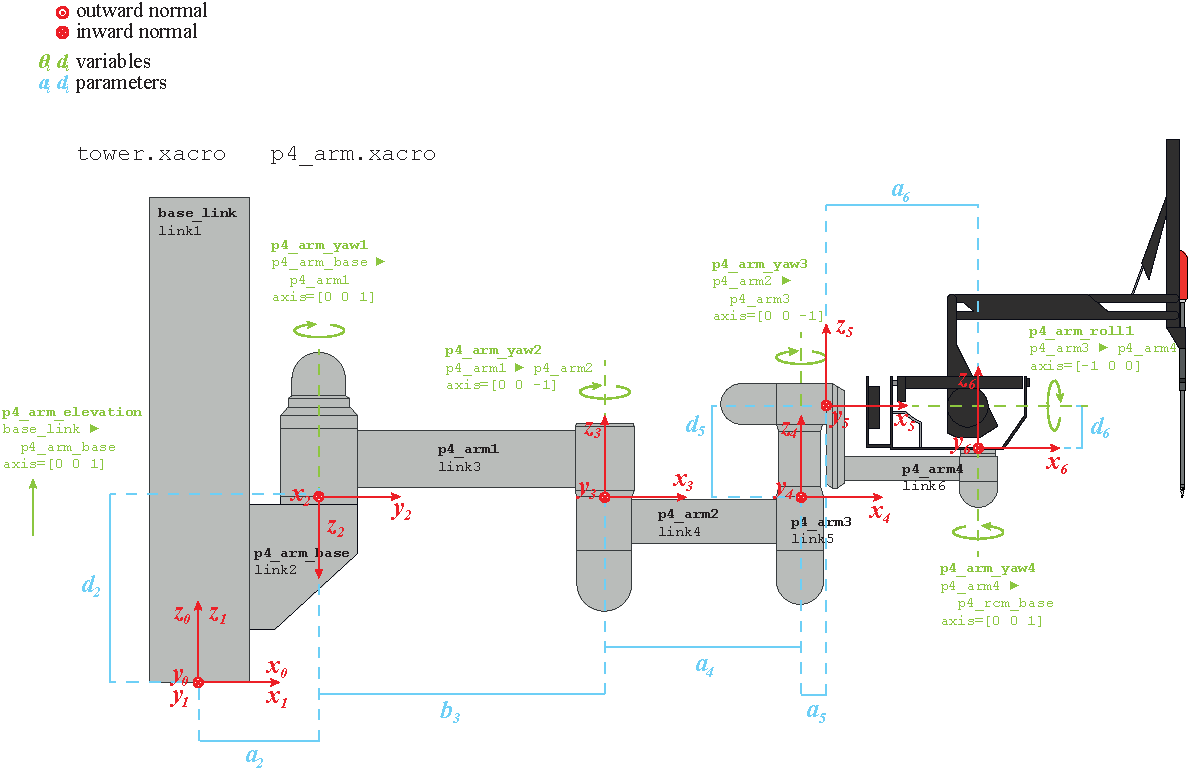
\includegraphics[width=1.1\textwidth]{p4_arm_xacro_frames.pdf}\label{fig:p4_arm_xacro_frames}}%
\vspace{5mm}\\
\hspace*{-15mm}
\subbottom[Coordinate frames for the joints on the robot hand and instrument.]{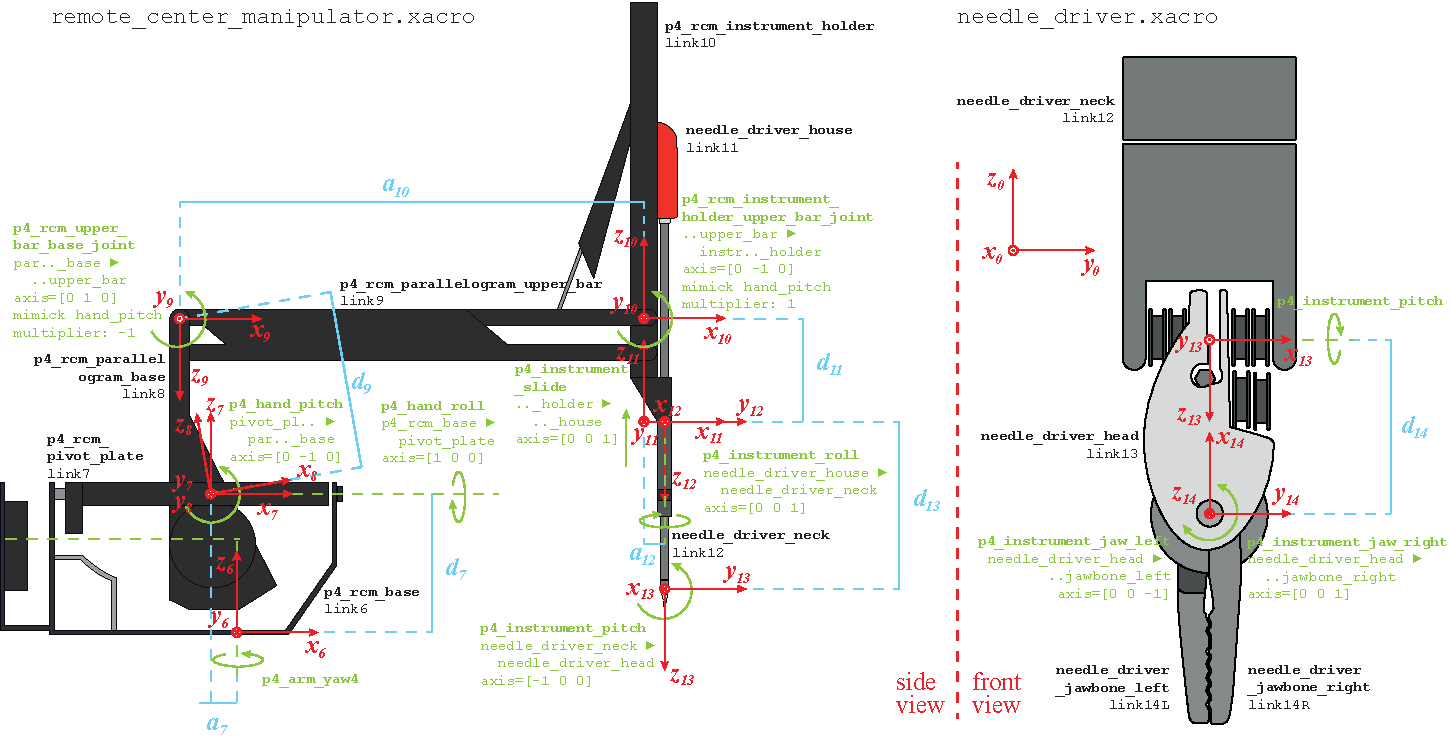
\includegraphics[width=1.15\textwidth]{p4_hand_xacro_frames.pdf}\label{fig:p4_hand_xacro_frames}}%
\caption{Orientation and position of coordinate frames $\Psi_0$, $\Psi_1$, ..., $\Psi_{14}$ according to the \gls{ros} \texttt{xacro} files.}
\label{fig:robot_xacro_frames}
\end{figure}

The position and orientation of the $i$th coordinate frame is given as a transformation matrix from the $i-1$th frame, where fixed distances and rotations are measured along/about the axes of the $i-1$th frame while free distances and rotations are measured along/about the axes of the $i$th frame. The parameters and variables shown in \autoref{fig:robot_xacro_frames} are given in \autoref{tab:xacro_param}.

\vspace{2mm}
\begin{table}[htbp]
\small
\centering
	\begin{tabular}{r | rrr c c l}\hline
		frame  & $a$ [m] & $b$ [m] & $d$ [m] & fixed rot. $\alpha$ [rad] & free rot. $\theta$ [rad] & name\\\hline
		1 & 0 & 0 & $d_1^*$ & $I$ & $I$ & \texttt{elevation}\\
		2 & 0.186 & 0 & 0.554 & $\textbf{R}_z(\pi/2)\textbf{R}_x(\pi)$ & $\textbf{R}_z(\theta_2^*)$ & \texttt{arm\_yaw1} \\
		3 & 0 & 0.583 & 0 & $\textbf{R}_z(\pi/2)\textbf{R}_x(-\pi)$ & $\textbf{R}_z(-\theta_3^*)$ & \texttt{arm\_yaw2} \\
		4 & 0.479 & 0 & -0.001 & $I$ & $\textbf{R}_z(-\theta_4^*)$ & \texttt{arm\_yaw3} \\
		5 & 0.057 & 0 & 0.198 & $I$ & $\textbf{R}_x(-\theta_5^*)$ & \texttt{arm\_roll1} \\
		6 & 0.352 & 0 & -0.117 & $I$ & $\textbf{R}_z(\theta_6^*)$ & \texttt{arm\_yaw4} \\
		7 & -0.042 & 0 & 0.161 & $I$ & $\textbf{R}_x(\theta_7^*)$ & \texttt{hand\_roll} \\
		8 & 0 & 0 & 0 & $\textbf{R}_y(-0.288)$ & $\textbf{R}_y(-\theta_8^*)$ & \texttt{hand\_pitch} \\
		9 & 0.011 & 0 & 0.186 & $\textbf{R}_y(0.288)\textbf{R}_x(\pi)$ & $\textbf{R}_y(-\theta_8)$ & \texttt{upper\_bar} \\
		10 & 0.520 & 0 & 0 & $\textbf{R}_x(\pi)$ & $\textbf{R}_y(-\theta_8)$ & \texttt{instrument\_holder} \\
		11 & 0 & 0 & -0.120 + $d_{11}^*$ & $I$ & $I$ & \texttt{instrument\_slide} \\
		12 & 0.052 & 0 & 0 & $\textbf{R}_z(\pi/2)\textbf{R}_x(\pi)$ & $\textbf{R}_z(\theta_{12}^*)$ & \texttt{instrument\_roll} \\
		13 & 0 & 0 & 0.177 & $I$ & $\textbf{R}_x(-\theta_{13}^*)$ & \texttt{instrument\_pitch} \\
		14L & 0 & 0 & 0.009 & $\textbf{R}_y(\pi/2)\textbf{R}_x(\pi/2)$ & $\textbf{R}_z(-\theta_{14L}^*)$ & \texttt{instrument\_jaw\_left} \\
		14\textbf{R} & 0 & 0 & 0.009 & $\textbf{R}_y(\pi/2)\textbf{R}_x(\pi/2)$ & $\textbf{R}_z(\theta_{14\textbf{R}}^*)$ & \texttt{instrument\_jaw\_right} \\
	\end{tabular}
	\caption{Variables (marked with $^*$) and parameters for the robot in \autoref{fig:robot_xacro_frames}. $I$ is the identity matrix (no rotation). Recent measures indicate that $d_2=0.812$, $a_2=0.198$, $a_4=0.435$, $\alpha_8=\textbf{R}_y(-0.07)$, $\alpha_9=\textbf{R}_y(0.07)\textbf{R}_x(\pi)$, $a_9=0$ and $d_\text{11,fixed}=0.188$ ($\Rightarrow$ $d_{12}=0.472$).}
	\label{tab:xacro_param}
\end{table}


I.e. according to \autoref{tab:xacro_param}, the transformation between frame 1 and 2 is given as:
\begin{equation}
^1_2\mathbf{T} = 
\begin{bmatrix}
\textbf{R}_z(\pi/2)\textbf{R}_x(\pi)\textbf{R}_z(\theta_2^*) & \mathbf{p}_2\\
0 & 1
\end{bmatrix}, \qquad\qquad
\mathbf{p}_2 = [0.186 \quad 0 \quad 0.554]^T
\end{equation}

The physical, low level controller and \gls{ros} limits for each of the variables are given in \autoref{tab:var_limits}

\vspace{2mm}
\begin{table}[htbp]
\small
\hspace*{-9mm}
%\begin{tabular}{l | cccccc}
%limits & $d_1^*$ & $\theta_2^*$ & $\theta_3^*$ & $\theta_4^*$ & $\theta_5^*$ & $\theta_6^*$ \\\hline
%physical & & & & & & \\
%\texttt{xacro} & [0, 1] & $\pm\pi/2$ & $\pm 2.8$ & $\pm 2.8$ & $\pm\pi/2$ & $\pm 2.8$
%\end{tabular}\\\\%
%\vspace{1mm}\\%
\begin{tabular}{l | ccccccc}\hline
limits & $\theta_7^*$ & $\theta_8^*$ & $d_{11}^*$ & $\theta_{12}^*$ & $\theta_{13}^*$ & $\theta_{14L}^*$ & $\theta_{14R}^*$ \\\hline
physical & $\pm$1.670 & [-0.951, 0.912] & [0.169, 0.410] & $\pm$4.712 & [-1.466, 1.536] & [-1.850, $\theta_{14\textbf{R}}^*$] & [$\theta_{14L}^*$, 1.702] \\
FPGA & [-1.333, 1.424] & [-0.812, 0.773] & [0.170, 0.409] & [-4.294, 4.416] & [-0.977, 0.908] & [-0.785, 1.335] & \\
\texttt{xacro} & $\pm\pi/2$ & [-0.8, 1] & $\pm$0.12 & $\pm3\pi/2$ & $\pm 1.5$ & $\pm 1.8$ & $\pm 1.8$
\end{tabular}
\normalsize
\caption{Limits on the (controllable) variables in \autoref{tab:xacro_param} and \autoref{fig:robot_xacro_frames}. The low level controller limits in the FPGA are set to avoid the physical limits, by switching off the motors on violation. The physical limits are measured limits.}
\label{tab:var_limits}
\end{table}
\vspace{2mm}

The first 6 degrees of freedom are elevation and rotation of the arm joints, and are manually set preoperatively and fixed, hence only the last 7 variables are controllable for trajectory planning. 
The frames are superimposed on the robot in \autoref{fig:robot_frames_pot}.

\vspace{-10mm}
\begin{figure}[htbp]
	\centering
\subbottom[\textbf{R}obot arm.]{\includegraphics[width=0.6\textwidth]{20150316_125233_red.pdf}\label{20150316_125233_red}}%
\hspace{5mm}
\subbottom[\textbf{R}obot arm.]{\includegraphics[width=0.25\textwidth]{20150316_125701_red.pdf}\label{20150316_125701_red}}%
\hspace{3mm}
\subbottom[\textbf{R}obot hand.]{\includegraphics[height=68mm]{20150316_140845_red.pdf}\label{20150316_140845_red}}%
\hspace{3mm}
\subbottom[Instr.]{\includegraphics[height=68mm]{20150317_110019_red.pdf}\label{20150317_110019_red}}%
\hspace{3mm}
\subbottom[Instr.]{\includegraphics[height=68mm]{20150317_111908_red.pdf}\label{20150317_111908_red}}%
\caption{Coordinate frame placement, distances and positive rotation direction for the robot arm, hand and instrument. In \autoref{20150316_125701_red} the positive rotation direction is shown for both \textbf{R}OS (green) and potentiometers (blue).}
\label{fig:robot_frames_pot}
\end{figure}

The position of the potentiometers measuring the joint variables 1-6 can be read from the interface to the secondary \gls{rio} as voltages. The scaling factor from these potentiometer voltages to the joint angle (in radians) are found through measurements and are given in \autoref{tab:arm_pot_factors}.
\vspace{2mm}
\begin{table}[H]
	\centering
\begin{tabular}{l | ccccc}
joint rotation [rad] & $\theta_2$, \texttt{yaw1} & $\theta_3$, \texttt{yaw2} & $\theta_4$, \texttt{yaw3} & $\theta_5$, \texttt{roll1} & $\theta_6$, \texttt{yaw4} \\
scaling factor [rad/V] & -0.225365326 & 0.302076216 & -0.306198114 & -0.311665937 & 0.314159265
\end{tabular}
\caption{Factor from potentiometer voltage measurements to arm joint angles.}
\label{tab:arm_pot_factors}
\end{table}



\newpage

\subsection{Testing Existing Kinematics in Matlab}
The single-axis rotation matrices are defined according to \autoref{eq:RxRyRz}

\begin{lstlisting}[language=matlab]
function rotation = rot(axis,angle)
	if axis==1
		rotation = [1 0 0; 0 cos(angle) -sin(angle); 0 sin(angle) cos(angle)];
	elseif axis==2
		rotation = [cos(angle) 0 sin(angle); 0 1 0; -sin(angle) 0 cos(angle)];
	elseif axis==3
		rotation = [cos(angle) -sin(angle) 0; sin(angle) cos(angle) 0; 0 0 1];
	end
end
\end{lstlisting}

The parameters are set according to \autoref{tab:xacro_param} (corrected according to measurements, see \autoref{tab:arm_pot_factors}) and the transformation matrices are computed as follows

\begin{lstlisting}[language=matlab]
%% Existing reference frames according to xacro files

% parameters: distances [m], a: along x, b: along y, d: along z
a = [0.0 0.198 0.0 0.435 0.057 0.352 -0.052 0.0 0.0 0.430 0.0 0.052 0.0 0.0 0.0];
b = [0 0 0.583 0 0 0 0 0 0 0 0 0 0 0 0];
d = [0 0.812 0 -0.001 0.198 -0.117 0.161 0 0.186 0 -0.104 0.0 0.177 0.009 0.009];

% parameters: rotations [rad]
R = [eye(3) rot(3,pi/2)*rot(1,pi) rot(3,pi/2)*rot(1,-pi) eye(3) eye(3) eye(3) eye(3) rot(2,-0.1745) rot(2,0.1745)*rot(1,pi) rot(1,pi) eye(3) rot(3,pi/2)*rot(1,pi) eye(3) rot(2,pi/2)*rot(1,pi/2) rot(2,pi/2)*rot(1,pi/2)];
for i = 1:length(a)
	Rot(:,:,i) = R(:,(i-1)*3+1:i*3);
end

% -----------------------------------------------------------------------
% variables: actuation axes
ax = [3 3 -3 -3 -1 3 1 -2 2 -2 3 3 -1 -3 3];

% first make the variable rotation matrices (assume all variables are angles)
for i = 1:length(a)
	Rot_var(:,:,i) = rot(abs(ax(i)),sign(ax(i))*state(i));
end
% eliminating the two rotations where the variable is a distance
Rot_var(:,:,1) = eye(3);
Rot_var(:,:,11) = eye(3);

% making the variable translation vectors
for i = 1:length(a)
	for j = 1:3
		if i == 1 || i == 11
			if j == abs(ax(i)) 
				p(j,i) = sign(ax(i))*state(i);
			end
		else
			p(j,i) = 0;
		end
	end
end

% Transformation matrices (forward kinematics)
for i = 1:length(a)
	fixed = [Rot(:,:,i) [a(i) b(i) d(i)]'; zeros(1,3) 1];
	free = [Rot_var(:,:,i) p(:,i); zeros(1,3) 1];
	Trans(:,:,i) = fixed*free;
end
\end{lstlisting}

To test the accuracy of the defined kinematics, computed distances are compared to measured distances. The results are shown in \autoref{tab:xacro_distances}, for different state configurations, with state = [state$_\text{arm}$, state$_\text{hand}$] $= [\{d_1, \theta_2, \theta_3, \theta_4, \theta_5, \theta_6\}, \{\theta_7, \theta_8, d_{11}, \theta_{12}, \theta_{13}, \theta_{14L}, \theta_{14R}\}]$ (as $\theta_8=\theta_9=\theta_{10}$, 9 and 10 are left out).

\begin{table}[htbp]
\small
\setlength{\tabcolsep}{4pt}
\centering
\subbottom[]{%
\begin{tabular}{l r r}\hline
dist. & calc. & meas.\\\hline
$|\,^6_7 p|$ & 16.92 & 16\\
$|\,^6_8 p|$ & 16.92 & 16\\
$|\,^6_9 p|$ & 35.43 & 34\\
$|\,^6_{10} p|$ & 55.52 & 53\\
$|\,^6_{11} p|$ & 49.75 & 51\\
$|\,^6_{12} p|$ & 54.36 & 52\\
$|\,^6_{13} p|$ & 49.18 & 47\\
$|\,^6_{14} p|$ & 49.07 & 47\\\hline
%$\,^0_{14} p_x$ & 202.27 & 210.0\\
%$\,^0_{14} p_y$ & 0 & 0\\
%$\,^0_{14} p_z$ & 94.62 & 92.0
$|\,^0_{14} p|$ & 231.49 & 229
\end{tabular}
\label{tab:state0}%
}\hfill
\subbottom[]{%
\begin{tabular}{l r r}\hline
dist. & calc. & meas.\\\hline
$|\,^6_7 p|$ & 16.92 & 16\\
$|\,^6_8 p|$ & 16.92 & 16\\
$|\,^6_9 p|$ & 29.72 & 27\\
$|\,^6_{10} p|$ & 39.53 & 36\\
$|\,^6_{11} p|$ & 45.42 & 44\\
$|\,^6_{12} p|$ & 49.57 & 46\\
$|\,^6_{13} p|$ & 60.15 & 65\\
$|\,^6_{14} p|$ & 60.77 & 66\\\hline
%$\,^0_{14} p_x$ & 221.01 & 220\\
%$\,^0_{14} p_y$ & 0.81 & 25\\
%$\,^0_{14} p_z$ & 106.65 & 96
$|\,^0_{14} p|$ & 243.72 & 241
\end{tabular}
\label{tab:state5}%
}\hfill
\subbottom[]{%
\begin{tabular}{l r r}\hline
dist. & calc. & meas.\\\hline
$|\,^6_7 p|$ & 16.92 & 16\\
$|\,^6_8 p|$ & 16.92 & 16\\
$|\,^6_9 p|$ & 33.81 & 31\\
$|\,^6_{10} p|$ & 44.99 & 46\\
$|\,^6_{11} p|$ & 44.71 & 49\\
$|\,^6_{12} p|$ & 49.82 & 50\\
$|\,^6_{13} p|$ & 53.64 & 53\\
$|\,^6_{14} p|$ & 53.99 & 54\\\hline
%$\,^0_{14} p_x$ & 147.41 & 156\\
%$\,^0_{14} p_y$ & 30.52 & 42\\
%$\,^0_{14} p_z$ & 104.72 & 98
$|\,^0_{14} p|$ & 185.16 & 189
\end{tabular}
\label{tab:state6}%
}\hfill
\subbottom[]{%
\begin{tabular}{l r r}\hline
dist. & calc. & meas.\\\hline
$|\,^6_7 p|$ & 16.92 & 16\\
$|\,^6_8 p|$ & 16.92 & 16\\
$|\,^6_9 p|$ & 31.66 & 32\\
$|\,^6_{10} p|$ & 62.96 & 65\\
$|\,^6_{11} p|$ & 53.98 & 55\\
$|\,^6_{12} p|$ & 56.84 & 56\\
$|\,^6_{13} p|$ & 44.05 & 42\\
$|\,^6_{14} p|$ & 43.49 & 41\\\hline
%$\,^0_{14} p_x$ & 175.48 & 177\\
%$\,^0_{14} p_y$ & 42.04 & 53\\
%$\,^0_{14} p_z$ & 103.19 & 94
$|\,^0_{14} p|$ & 217.15 & 207
\end{tabular}
\label{tab:state7}%
}\hfill
\setlength{\tabcolsep}{6pt}
\caption{Calculated and measured distances [cm] between frame origins. In \ref{tab:state0} all variables are set to zero. In \ref{tab:state5} state$_\text{hand}=$[1.3, 0.7, -0.05, 0, 0, -0.23, 0]. In \ref{tab:state6} state = [\{0, 0.2, 0.5, -1.4, 0, 0.8\}, \{-0.5, 0.5, 0.03, 0, 0, -0.2, 0\}]. In \ref{tab:state7} state = [\{0, -0.2, -0.6, 0.9, 0, 0.4\}, \{-0.6, -0.6, 0, 0, 0, -0.2, 0\}].}
\label{tab:xacro_distances}
\end{table}

% % state 7


%\vspace*{-3mm}
\section{Defining Kinematics According to Denavit-Hartenberg Convention}\label{sec:denavit_hartenberg}
\vspace{-2mm}
In order to simplify calculations, the robot coordinate frame convention \gls{dh} is adapted, and a new set of coordinate frames and transformation matrices are established. According to the \gls{dh} convention a frame is placed such that
\begin{itemize}
\itemsep-1.3mm 
\item frame $i$ is fixed with respect to link $i$
\item the $z_i$ axis is aligned with link $i+1$ actuation axis
\item variable/parameter $\theta_i$ is the angle from $x_{i-1}$ to $x_i$ about $z_{i-1}$
\item variable/parameter $d_i$ is the distance from origin $i-1$ to $x_i$ measured along $z_{i-1}$
\item parameter $a_i$ is the distance from $z_{i-1}$ to $z_i$ measured along $x_i$
\item parameter $\alpha_i$ is the angle from $z_{i-1}$ to $z_i$ about $x_i$
\end{itemize}

Using this convention, all transformations between frames can be written on the form
\begin{equation}
\hspace*{-2mm}
\small
^{i-1}_i T = %T_{rot\,z,\theta_i} T_{trans\,z,d_i} T_{trans\,x,a_i} T_{rot\,x,\alpha_i} =
\begin{bmatrix}
\textbf{R}_z(\theta_i) & \begin{bmatrix}0\\ 0\\ d_i\end{bmatrix}\\
0 & 1
\end{bmatrix}
\begin{bmatrix}
\textbf{R}_x(\alpha_i) & \begin{bmatrix}a_i\\ 0\\ 0\end{bmatrix}\\
0 & 1
\end{bmatrix}
=
\begin{bmatrix}
\cos(\theta_i) & -\cos(\alpha_i)\sin(\theta_i) & \sin(\alpha_i)\sin(\theta_i) & a_i \cos(\theta_i)\\
\sin(\theta_i) & \cos(\alpha_i)\cos(\theta_i) & -\sin(\alpha_i)\cos(\theta_i) & a_i \sin(\theta_i)\\
0 & \sin(\alpha_i) & \cos(\alpha_i) & d_i\\
0 & 0 & 0 & 1
\end{bmatrix}
\end{equation}

The placement of coordinate frames according to the \gls{dh} convention is shown in \autoref{fig:robot_DH_frames} and the parameters used for this set of frame transformations are given in \autoref{tab:DH_param}.


\begin{figure}[htbp]
	\vspace*{-10mm}
	\hspace{-10mm}
	\subbottom[Coordinate frames for the joints on the robot arm.]{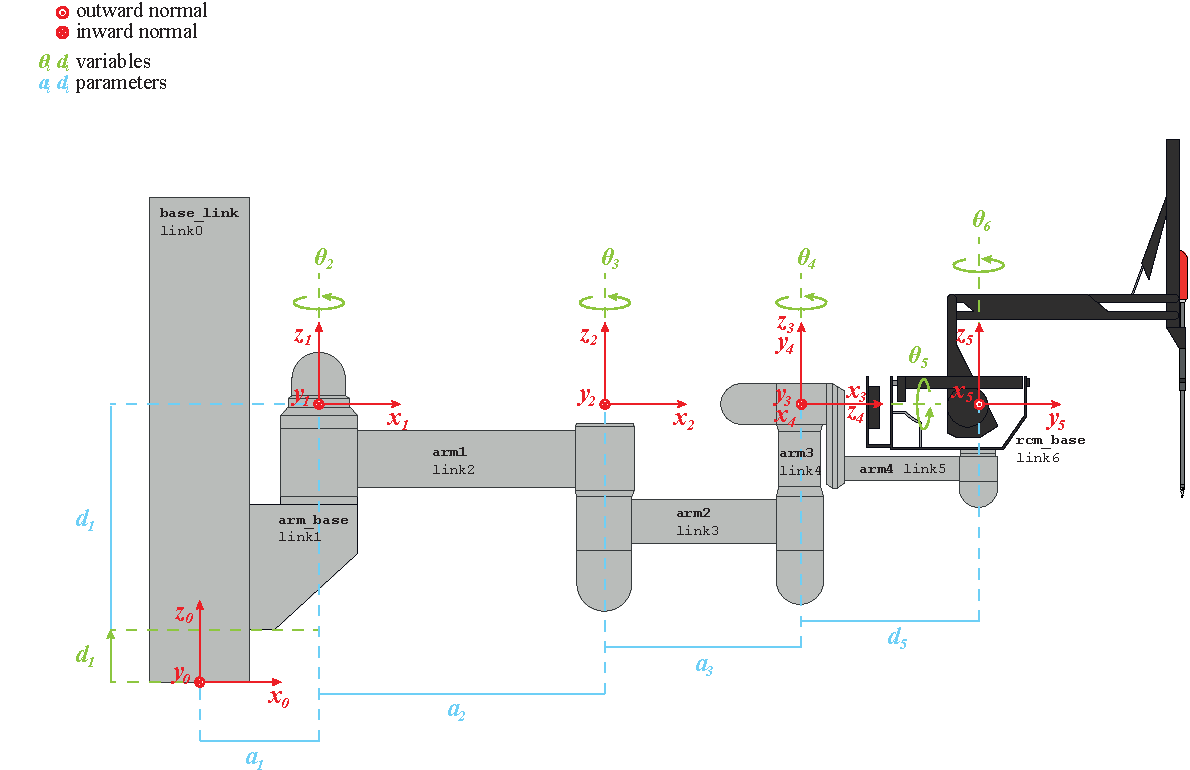
\includegraphics[width=1.1\textwidth]{p4_arm_DH_frames.pdf}\label{fig:p4_arm_DH_frames}}%
	\vspace{5mm}\\
	\hspace*{-15mm}
	\subbottom[Coordinate frames for the joints on the robot hand and instrument.]{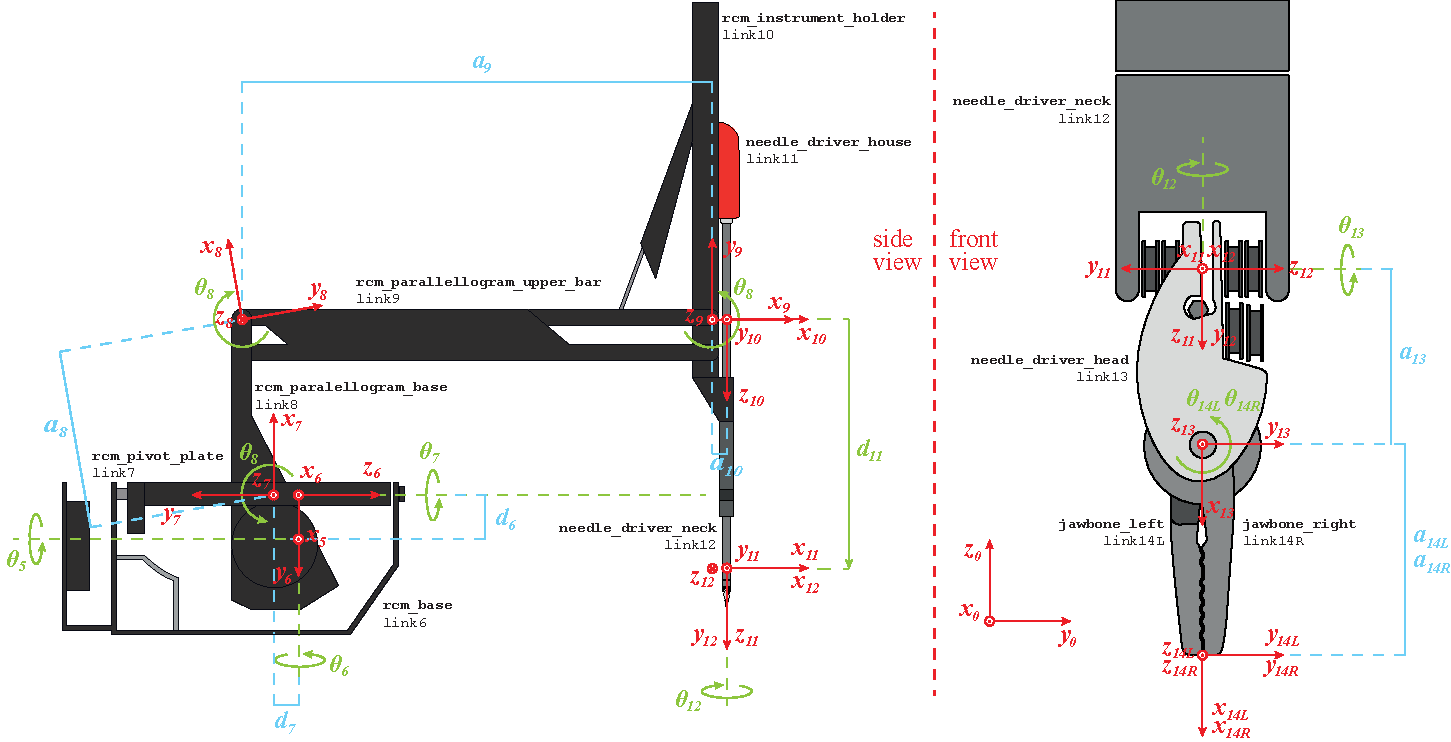
\includegraphics[width=1.15\textwidth]{p4_hand_DH_frames.pdf}\label{fig:p4_hand_DH_frames}}%
	\caption{Orientation and position of coordinate frames $\Psi_0$, $\Psi_1$, ..., $\Psi_{14}$ defined according to the \gls{dh} convention.}
	\label{fig:robot_DH_frames}
\end{figure}

\begin{table}[htbp]
	\small
	\vspace*{-3mm}
	\centering
	\begin{tabular}{r | rrrr}\hline
		$i$  & $\theta_i$ [rad]& $d_i$ [m] & $a_i$ [m] & $\alpha_i$ [rad] \\\hline
		1 & 0 &  $0.453+d_1^*$ & 0.198 & 0 \\
		2 & $\theta_2^*$ & 0 & 0.582 & 0 \\
		3 & $\theta_3^*$ & 0 & 0.435 & 0\\
		4 & $\pi/2+\theta_4^*$ & 0 & 0 & $\pi/2$\\
		5 & $\pi+\theta_5^*$ & 0.412 & 0 & $\pi/2$ \\
		6 & $\theta_6^*$ & 0.047 & 0 & $-\pi/2$ \\
		7 & $-\pi/2+\theta_7^*$ & -0.035 & 0 & $-\pi/2$ \\
		8 & $0.03+\theta_8^*$ & 0 & 0.190 & $\pi$ \\
		9 & $0.03+\pi/2+\theta_8^*$ & 0 & 0.515 & $\pi$ \\
		10 & $\theta_8^*$ & 0 & 0.040 & $\pi/2$\\
		11 & 0 & $0.282+d_{11}^*$ & 0  & 0 \\
		12 & $\theta_{12}^*$ & 0 & 0 & $\pi/2$ \\
		13 & $\pi/2+\theta_{13}^*$ & 0 & 0.009 & $\pi/2$ \\
		14L & $\theta_{14L}^*$ & 0 & 0.009 & 0\\
		14R & $\theta_{14R}^*$ & 0 & 0.009 & 0 \\
	\end{tabular}
	\caption{Variables (marked with $^*$) and parameters for the robot in \autoref{fig:robot_DH_frames} defined according to the \gls{dh} convention, where $\theta_i$ and $d_i$ are rotation/translation along $z_{i-1}$, while $a_i$ and $\alpha_i$ are translation/rotation along $x_i$.}
	\label{tab:DH_param}
\end{table}

\subsection{Testing \gls{dh} Kinematics in Matlab}
The new transformation matrices are computed and tested similarly, to determine the accuracy of the defined robot kinematics, and the results are seen in \autoref{tab:DH_distances}.
\begin{lstlisting}[language=matlab]
%% Coordinate frames defined according to Denavit-Hartenberg convention
% Parameters
a_fix = [0.198 0.5820 0.435 0 0 0 0 0.1900 0.515 0.0400 0 0 0.0095 0.0095 0.0095];
d_fix = [1 0 0 0 0.4122 0.0474 -0.0450 0 0 0 0.282 0 0 0 0];
alpha = [0 0 0 pi/2 pi/2 -pi/2 -pi/2 pi pi pi/2 0 pi/2 pi/2 0 0];
theta_fix = [0 0 0 pi/2 pi 0 -pi/2 10/180*pi 10/180*pi+pi/2 0 0 0 pi/2 0 0];

% Variables (signs are included as long as state comes from old frame convention)
d_free = [d1 0 0 0 0 0 0 0 0 0 -d11 0 0 0 0];
theta_free = [0 -th2 -th3 -th4 -th5 th6 th7 th8 th8 th8 0 th12 -th13 th14L -th14R];

% Transformation matrices
for i = 1:length(a_fix)
	Tz = [rot(3,theta_free(i)+theta_fix(i)) [0;0;d_free(i)+d_fix(i)]; zeros(1,3) 1];
	Tx = [rot(1,alpha(i)) [a_fix(i);0;0]; zeros(1,3) 1];
	T_DH(:,:,i) = Tz*Tx;
end
\end{lstlisting}

\begin{table}[htbp]
\small
\setlength{\tabcolsep}{4pt}
\centering
\subbottom[]{%
\begin{tabular}{l r r}\hline
dist. & calc. & meas.\\\hline
$|\,^5_6 p|$ & 4.74 & 5\\
$|\,^5_7 p|$ & 6.54 & 7\\ %6\\
$|\,^5_8 p|$ & 24.71 & 24\\
$|\,^5_9 p|$ & 49.60 & 49\\
$|\,^5_{10} p|$ & 53.15 & 53\\ %52\\
$|\,^5_{11} p|$ & 47.94 & 48\\
$|\,^5_{12} p|$ & 47.94 & 48\\
$|\,^5_{13} p|$ & 48.04 & 48\\
$|\,^5_{14} p|$ & 48.16 & 48\\\hline
%$\,^0_{14} p_x$ & 210.42 & 210\\
%$\,^0_{14} p_y$ & 0 & 0\\
%$\,^0_{14} p_z$ & 93.35 & 92
$|\,^0_{14} p|$ & 230.20 & 229
\end{tabular}
\label{tab:state0dh}%
}\hfill
\subbottom[]{%
\begin{tabular}{l r r}\hline
dist. & calc. & meas.\\\hline
$|\,^5_6 p|$ & 4.74 & 5\\ %4\\
$|\,^5_7 p|$ & 6.54 & 7\\ %8\\
$|\,^5_8 p|$ & 23.79 & 24\\ %20\\
$|\,^5_9 p|$ & 35.40 & 34\\ %33\\
$|\,^5_{10} p|$ & 39.20 & 39\\ %49\\
$|\,^5_{11} p|$ & 57.82 & 64\\ %66\\
$|\,^5_{12} p|$ & 57.82 & 64\\ %66\\
$|\,^5_{13} p|$ & 58.54 & 67\\ %65\\
$|\,^5_{14} p|$ & 59.23 & 68\\ \hline %66\\
%$\,^0_{14} p_x$ & 230.81 & 220\\
%$\,^0_{14} p_y$ & 1.88 & 25\\
%$\,^0_{14} p_z$ & 107.03 & 96
$|\,^0_{14} p|$ & 243.20 & 241
\end{tabular}
\label{tab:state5dh}%
}\hfill
\subbottom[]{%
\begin{tabular}{l r r}\hline
dist. & calc. & meas.\\\hline
$|\,^5_6 p|$ & 4.74 & 5\\ %6\\
$|\,^5_7 p|$ & 6.54 & 7\\ %8\\
$|\,^5_8 p|$ & 25.14 & 24\\ %19\\
$|\,^5_9 p|$ & 39.04 & 40\\ %37\\
$|\,^5_{10} p|$ & 43.02 & 42\\ %41\\
$|\,^5_{11} p|$ & 51.33 & 51\\ %54\\
$|\,^5_{12} p|$ & 51.33 & 51\\ %54\\
$|\,^5_{13} p|$ & 51.86 & 52\\ %55\\
$|\,^5_{14} p|$ & 52.40 & 52\\\hline %55\\
%$\,^0_{14} p_x$ & 150.05 & 156\\
%$\,^0_{14} p_y$ & 39.71 & 42\\
%$\,^0_{14} p_z$ & 103.79 & 98
$|\,^0_{14} p|$ & 184.99 & 189
\end{tabular}
\label{tab:state6dh}%
}\hfill
\subbottom[]{%
\begin{tabular}{l r r}\hline
dist. & calc. & meas.\\\hline
$|\,^5_6 p|$ & 4.74 & 5\\
$|\,^5_7 p|$ & 6.54 & 7\\ %8\\
$|\,^5_8 p|$ & 21.65 & 22\\ %24\\
$|\,^5_9 p|$ & 58.87 & 58\\ %56\\
$|\,^5_{10} p|$ & 61.22 & 61\\ %59\\
$|\,^5_{11} p|$ & 42.53 & 41\\ %39\\
$|\,^5_{12} p|$ & 42.53 & 41\\ %39\\
$|\,^5_{13} p|$ & 42.08 & 40\\ %38\\
$|\,^5_{14} p|$ & 41.67 & 40\\\hline %38\\
%$\,^0_{14} p_x$ & 183.40 & 177\\
%$\,^0_{14} p_y$ & 44.76 & 53\\
%$\,^0_{14} p_z$ & 103.27 & 94
$|\,^0_{14} p|$ & 216.08 & 207
\end{tabular}
\label{tab:state7dh}%
}\hfill
\setlength{\tabcolsep}{6pt}
\caption{Calculated and measured distances [cm] between frame origins. The same states are used as given in \autoref{tab:xacro_distances}.}
\label{tab:DH_distances}
\end{table}

%%% STATE5


\section{Defining da Vinci Kinematics for Active Joints}\label{sec:app_activejoints_kinematics}
As the kinematics described via the \texttt{xacro} files implement translations first, and then RPY rotations (extrinsic roll (about $x$-axis), pitch (about $y$-axis), yaw (about $z$-axis) rotation), the DH convention cannot be implemented directly in the robot kinematics through the joint description in the \texttt{xacro} files. Furthermore, the convention here is that each frame (joint) is fixed in its child link (corresponding to the fixed rotations preceding the free rotation), and not in its parent link as in the DH convention.

A compromise is made, defining a new set of frames for the \texttt{xacro} kinematics, adhering to the \gls{dh} constraint that each free rotation/translation is about/along the local $z$-axis. Furthermore, for convenience of the inverse kinematics solver, the two passive joints mimicking the hand pitch movement are removed from the kinematic chain, also removing a series of links (marked with grey in \autoref{fig:p4_hand_compromise_frames}). For convenience of placing the hand roll and pitch frames in the pivot point, a virtual link is inserted in the \texttt{xacro} file after each of these two joints. 

Transformation matrices describing the kinematics of the \texttt{xacro} files are written on the form
\begin{equation}
\hspace*{-2mm}
\small
^{i-1}_i T =
\begin{bmatrix}
\textbf{R}_z(\text{yaw})\textbf{R}_y(\text{pitch})\textbf{R}_x(\text{roll}) & \begin{bmatrix}a_i\\ b_i\\ d_i\end{bmatrix}\\
0 & 1
\end{bmatrix}
\begin{bmatrix}
\textbf{R}_z(\theta_i^*) & \begin{bmatrix}0\\ 0\\ d_i^* \end{bmatrix}\\
0 & 1
\end{bmatrix}
\label{eq:xacro_transformation}
\end{equation}
where the transformation described in $^{i-1}_i T$ is implemented in joint $i$ in the \texttt{xacro} file  as (for joint 8)
\begin{lstlisting}[language=xml]
  <joint name="p4_hand_pitch"  type="revolute">
  <origin
  		xyz="0 0 0"
  		rpy="1.5708 0 0" />
  <parent link="rcm_vitual0" />
  <child link="rcm_vitual1" />
  <axis xyz="0 0 1" />
  ...
  </joint>
\end{lstlisting}
The measures for all translations and rotations are displayed in \autoref{tab:compromise_param}.

\vspace{2mm}
\begin{table}[htbp]
\small
\centering
\begin{tabular}{r | rrr | ccc | c l}\hline
 & \multicolumn{3}{c|}{fixed translation  [m]} & \multicolumn{3}{c|}{fixed rotation [rad]} & freedom & \\
frame  & $a$ ($x$)  & $b$ ($y$)  & $d$ ($z$)  & roll  & pitch & yaw & $\theta^*$ or $d^*$ & joint name\\\hline
1 & 0 & 0 & 0.998 & 0 & 0 & 0 & $d_1^*$ & \texttt{elevation}\\
2 & 0.198 & 0 & 0 & 0 & 0 & 0 & $\theta_2^*$ & \texttt{arm\_yaw1} \\
3 & 0.582 & 0 & 0 & 0 & 0 & 0 & $\theta_3^*$ & \texttt{arm\_yaw2} \\
4 & 0.435 & 0 & 0 & 0 & 0 & 0 & $\theta_4^*$ & \texttt{arm\_yaw3} \\
5 & 0 & 0 & 0 & 0 & $\pi/2$ & 0 & $\theta_5^*$ & \texttt{arm\_roll1} \\
6 & 0 & 0 & 0.412 & 0 & $-\pi/2$ & 0 & $\theta_6^*$ & \texttt{arm\_yaw4} \\
7 & 0.482 & 0 & 0.047 & 0 & $\pi/2$ & 0 & $\theta_7^*$ & \texttt{hand\_roll} \\
8 & 0 & 0 & 0 & $\pi/2$ & 0 & 0 & $\theta_8^*$ & \texttt{hand\_pitch} \\
9 & 0.097 & 0 & 0 & 0 & $-\pi/2$ &  0 & $d_9^*$ & \texttt{instrument\_slide} \\
10 & 0 & 0 & 0 & 0 & 0 & 0 & $\theta_{10}^*$ & \texttt{instrument\_roll} \\
11 & 0 & 0 & 0 & 0 & $\pi/2$ & 0 & $\theta_{11}^*$ & \texttt{instrument\_pitch} \\
12L & 0.009 & 0 & 0 & $-\pi/2$ & 0 & 0 & $\theta_{12L}^*$ & \texttt{instrument\_jaw\_left} \\
12R & 0.009 & 0 & 0 & $-\pi/2$ & 0 & 0 & $\theta_{12R}^*$ & \texttt{instrument\_jaw\_right} \\
	\end{tabular}
	\caption{Fixed translations and rotations implemented via \texttt{xacro} as described in \autoref{eq:xacro_transformation}, followed by a free rotation or translation about the (new) $z$-axis.}
	\label{tab:compromise_param}
\end{table}



\begin{figure}[htbp]
	\vspace*{-10mm}
	\hspace{-10mm}
	\subbottom[Coordinate frames for the joints on the robot arm.]{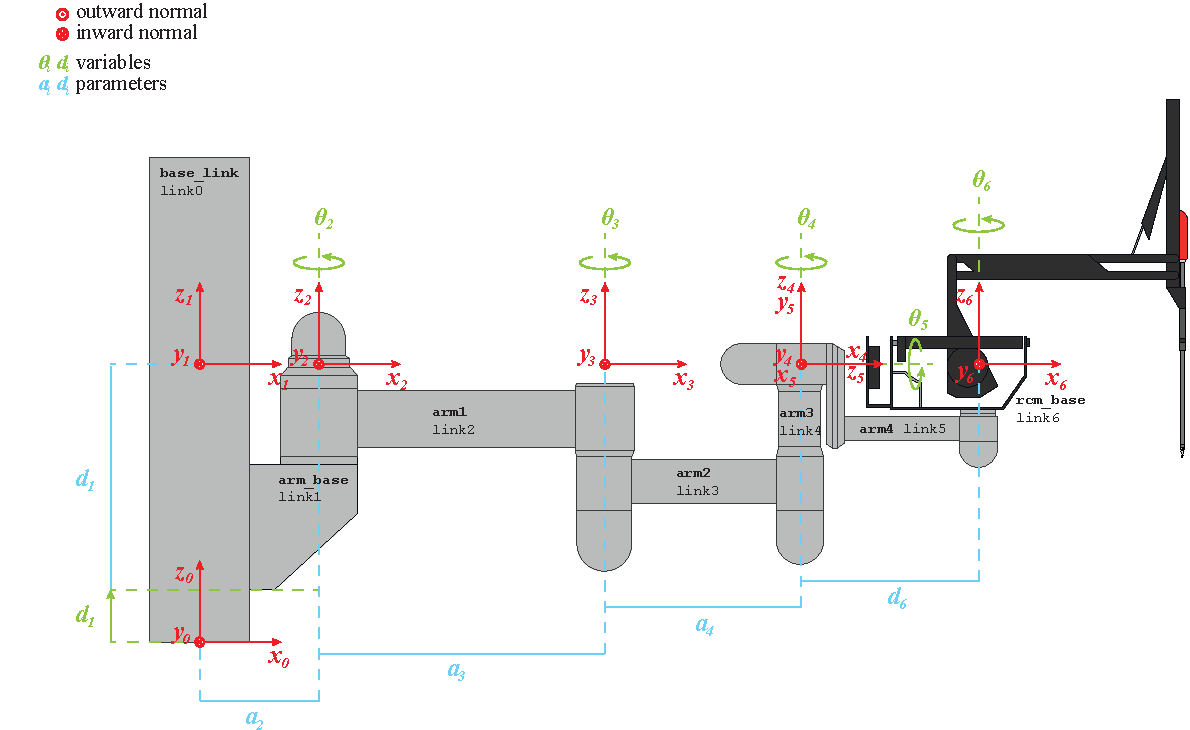
\includegraphics[width=1.1\textwidth]{p4_arm_compromise_frames.pdf}\label{fig:p4_arm_compromise_frames}}%
	\vspace{5mm}\\
	\hspace*{-15mm}
	\subbottom[Coordinate frames for the joints on the robot hand and instrument.]{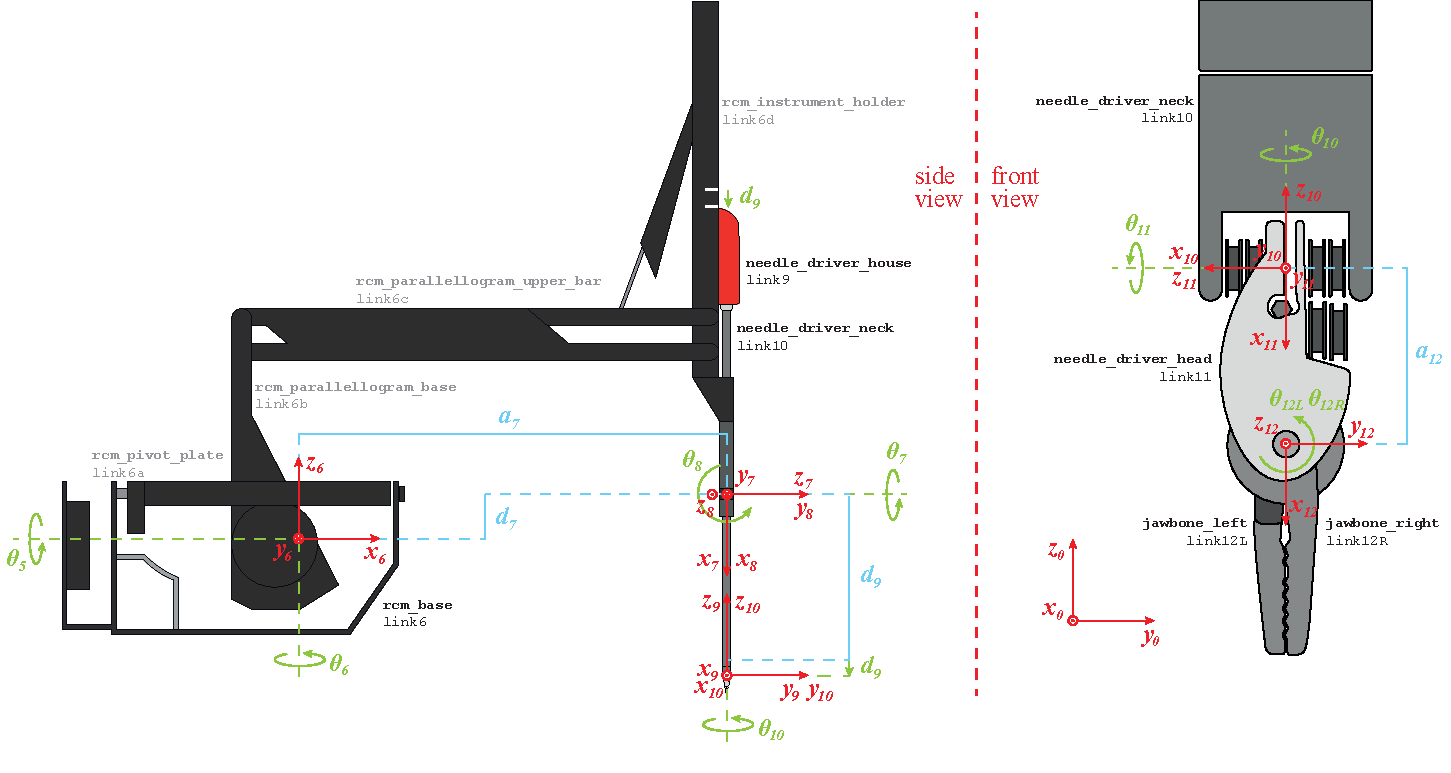
\includegraphics[width=1.15\textwidth]{p4_hand_compromise_frames.pdf}\label{fig:p4_hand_compromise_frames}}%
	\caption{Orientation and position of coordinate frames $\Psi_0$, $\Psi_1$, ..., $\Psi_{12}$ defined according to the compromise between the \gls{dh} convention and the \texttt{xacro} convention.}
	\label{fig:robot_compromise_frames}
\end{figure}

\subsection{Testing Active Joint Kinematics in Matlab}
As for the previous sets of coordinate frames, the transformations are tested in Matlab to check the conformity with the two other kinematic chains.

\begin{lstlisting}[language=matlab]
%% Coordinate frames defined as a compromise between DH and the xacro syntax, excluding passive joints
% parameters: distances [m], and rotations [rad]
a = [0 0.198 0.582 0.435 0 0 0.482 0 0.097 0 0 0.009 0.009];
d = [0.998 0 0 0 0 0.412 0.047 0 0 0 0 0 0];
roll = [0 0 0 0 0 0 0 pi/2 0 0 0 -pi/2 -pi/2];
pitch = [0 0 0 0 pi/2 -pi/2 pi/2 0 -pi/2 0 pi/2 0 0];

% Variables (signs are included as long as state comes from old frame convention)
d_free = [d1 0 0 0 0 0 0 0 -d11 0 0 0 0];
theta_free = [0 -th2 -th3 -th4 -th5 th6 th7 th8 0 th12 -th13 th14L -th14R];

% Transformation matrices (forward kinematics)
for i = 1:length(a)
	fixed = [rot(2,pitch(i))*rot(1,roll(i)) [a(i) 0 d(i)]'; zeros(1,3) 1];
	free = [rot(3,theta_free(i)) [0 0 d_free(i)]'; zeros(1,3) 1];
	Trans(:,:,i) = fixed*free;
end
\end{lstlisting}

The new frame transformations result in a set of calculated distances corresponding relatively well to the measured distances, as seen in \autoref{tab:compromise_distances}.

\begin{table}[htbp]
	\centering
\begin{tabular}{l | r r r r}\hline
state as in & table \ref{tab:state0} & table \ref{tab:state5} & table \ref{tab:state6} & table \ref{tab:state7}\\\hline
calculated distance & 2.31\,m & 2.38\,m & 1.85\,m & 2.17\,m\\
measured distance & 2.29\,m & 2.41\,m & 1.89\,m & 2.07\,m\\
\end{tabular}
\caption{Calculated and measured distances between origin of the inertial and the tool tip frames, when using the the active joint kinematics for the calculations.}
\label{tab:compromise_distances}
\end{table}


\textcolor{white}{\gls{rpy}}
